
%%%%%%%%%%%%%%%%%%%%%%%%%%%%%%%%%%%%%%%%%%%%%%%%%%%%%%%%%%%%%%%%%%%%%%%%%%%%%%
%%%%%%%%%%%%%%%%%%%%%%%%%%%%%%%%%%%%%%%%%%%%%%%%%%%%%%%%%%%%%%%%%%%%%%%%%%%%%% 

%\section{Introduction}
%\label{sec: Introduction}%

\emph{Microfluidics} is an area of science and engineering dedicated to the study and 
manipulation of very small (picoliter to nanoliter~\cite{hsieh2012reagent}) amounts of 
fluids. Research advances in microfluidics led to the development of 
\emph{lab-on-chip} ($\LoC$) devices that integrate on a small chip
various functions of bulky and costly biochemical systems, including 
dispensing, mixing, and filtering of fluids, particle separation, and detection of chemicals.
$\LoC$s play increasingly important roles in applications that include
cancer research~\cite{li2013probing}, 
environment monitoring~\cite{marle2005microfluidic}, 
protein analysis~\cite{xu2010defect}, 
drug discovery~\cite{einav2008discovery} and physiological 
sample analysis~\cite{srinivasan2004integrated}.
The importance of $\LoC$ devices will soon scale up with the introduction of 
\emph{cloud laboratories}~\cite{hayden2014automated}, 
which give researchers access to state-of-the-art equipment and data analysis tools and
allow them to carry out their experiments remotely.

One of the most fundamental functions of $\LoC$ devices is \emph{mixing} of different fluids.
In particular, in applications related to sample preparation,
the objective is to produce desired volumes of pre-specified mixtures of fluids.
In typical applications only two fluids are involved, in which case
the process of mixing is often referred to as \emph{dilution}. The
fluid to be diluted is called \emph{reactant} and the diluting fluid is called \emph{buffer}.
For example, in clinical diagnostics common reactants include blood, serum, plasma and urine, while
phosphate buffered saline is often used as buffer~\cite{srinivasan2004integrated}.

There is a variety of different technologies that can be used to manufacture 
microfluidic devices for fluid mixing. In our work, we consider microfluidic
chips that involve a collection of tiny components called \emph{micro-mixers} connected
by \emph{micro-channels}. In such chips, input fluids are injected into the chip using fluid dispensers,
then they travel, following appropriate micro-channels, through a sequence of micro-mixers
in which they are subjected to mixing operations, and are eventually discharged into output reservoirs. 
We focus on \emph{droplet-based} chips, where fluids are manipulated in discrete units called \emph{droplets}. 
In such chips each micro-mixer has exactly two input and two output channels. 
It receives one droplet of fluid from
each input, mixes them perfectly, producing two identical droplets on its outputs.
Specifically, if the input droplets have (reactant) concentrations
$a,b$, then the produced droplets will have concentration $\half(a+b)$. 
It follows that all droplets flowing through the chip have concentrations
of the form $c/2^d$, where $c$ and $d\ge 0$ are integers. 
This simply means that their binary representations are finite, and we will
refer to such numbers simply as \emph{binary numbers}.
Throughout the paper we will assume (often tacitly) that
all concentration values are binary numbers. In this representation,
the number $d$, called \emph{precision}, is the number of
fractional bits (assuming $c$ is odd when $d\ge 1$). 

Processing of droplets on such chips can be naturally represented by a
directed acyclic graph $G$ that we call a \emph{mixing graph}. The edges of $G$
represent micro-channels. Source vertices (with in-degree $0$ and out-degree $1$) represent
dispensers, internal vertices (with in-degree and out-degree $2$)
represent micro-mixers, and sink vertices (with in-degree $1$ and out-degree $0$) represent
output reservoirs. Given a set $I$ of input droplets injected into the source nodes,
$G$ will convert it into a set $T$ of droplets in its sink nodes. We refer to this set $T$
as a \emph{target set}. 
An example of a mixing graph is shown in Figure~\ref{fig: mixing graph example}.
Here, and elsewhere in the paper, we represent each
droplet by its reactant concentration (which uniquely determines the 
buffer concentration, as both values add up to $1$).

%%%%%%
	
\begin{figure}[ht]
	\begin{center}
		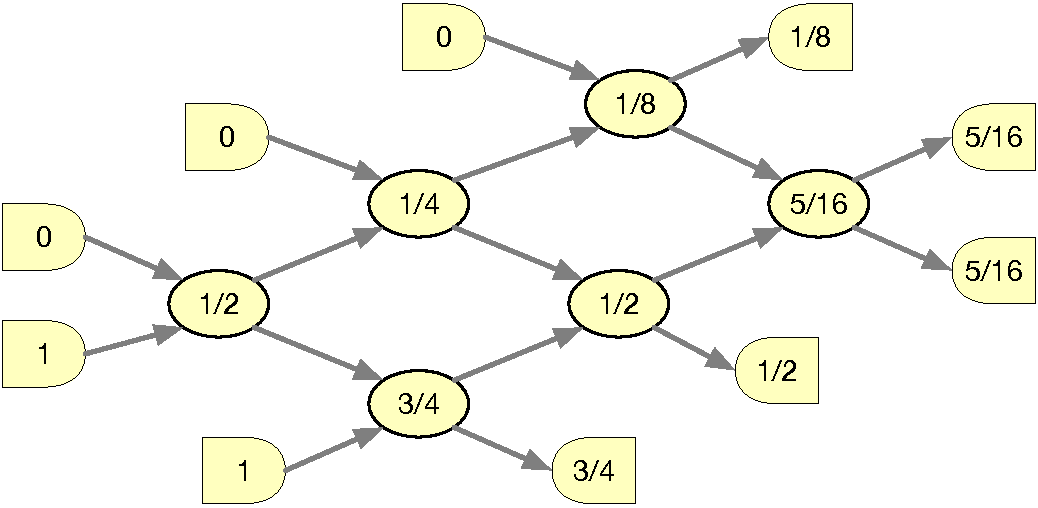
\includegraphics[width = 3.2in]{mixing_graph_example.pdf}
		\caption{A mixing graph that produces 
		target set $T = \braced{\oneeighth,\fivesixteenths,\fivesixteenths,\onehalf,\threefourths}$
		from input set $I = \braced{0,0,0,1,1}$.
		Numbers on the micro-mixers (internal nodes) represent droplet concentrations produced
		by these mixers.}
		\label{fig: mixing graph example}
	\end{center}
\end{figure}

There is growing literature in the embedded systems and bioengineering communities
on designing microfluidic chips  represented by such mixing graphs.
The most fundamental algorithmic problem emerging in this
area is the following:

\begin{description}
	\item{{\MixReachability:}}
Given an input set $I$ and a target set $T$ of droplets with given reactant concentrations, 
design (if at all possible) a mixing graph that converts $I$ into $T$.
\end{description}

If there is a mixing graph that converts $I$ into $T$ then we say that 
$T$ is \emph{mix-reachable}, or just \emph{reachable}, from $I$.  
For $T$ to be reachable from $I$, clearly, $I$ and $T$ must have the
same cardinality and equal reactant volumes. However,  these conditions
are not sufficient. For example, $T = \braced{\onefourth,\threefourths}$
is not reachable from $I = \braced{0,1}$ (or from any other input set consisting only
of pure buffer and reactant droplets), because producing $\onefourth$ 
requires at least
two buffer droplets and one reactant droplet, but $T$ itself contains only two droplets.
 
In typical applications the input set $I$ consists of pure
reactant and buffer droplets (that is, only $0$'s and $1$'s). 
We denote this variant by {\MixProducibility}, and target sets reachable from such input
sets are caled \emph{mix-producible}, or just \emph{producible}.
{\MixProducibility} is not likely to be computationally easier than  {\MixReachability}. 
If $\calA$ is an algorithm that solves {\MixProducibility} then, via a simple linear
mapping, it can also solve the variant of {\MixReachability} where the input set
has droplets of \emph{any} two given concentrations (instead of $0$ and $1$). 
Further, consider the family $\braced{C_i}$ of concentration sets produced by up to 
some constant number $k$ of mixing operations from $I$. Then $\calA$ in fact determines whether $T$ is reachable
from at least one $C_i$, yet these sets $C_i$ have up to $k+2$ different
concentrations. While we do not have a formal reduction, these properties indicate that
taking advantage of
the special form of inputs in {\MixProducibility} may be challenging.

%%%%%%%%%%%%


\myparagraph{Related work} 
The previous work in the literature focuses on designing mixing graphs that dilute the reactant
to produce some desired concentrations -- that is on the {\MixProducibility} problem.
To generate target sets that are not producible, one can consider mixing
graphs that besides a target set $T$ also produce some amount of superfluous fluid
called \emph{waste}. If we allow waste then, naturally, {\MixProducibility} can be extended 
to an optimization problem where the objective is to design a
mixing graph that generates $T$ while minimizing waste. Alternative
objective functions have been studied, for example minimizing the
reactant waste, minimizing the number of micro-mixers, and other.

Most of the previous papers on this topic study designing mixing graphs using
heuristic approaches. Earlier studies
focused on producing \emph{single-concentration targets}, where only one droplet of some 
desired concentration is needed. 
This line of research was pioneered by Thies~{\etal}~\cite{thies2008abstraction},
who proposed an algorithm  called $\MinMix$ 
that constructs a mixing graph for a single target droplet.
Roy~{\etal}~\cite{roy2010optimization} developed a single-droplet
algorithm called $\DMRW$ that considered waste reduction and the number of mixing operations.
Huang~{\etal}~\cite{huang2012reactant} and Chiang~{\etal}~\cite{chiang2013graph}
proposed single-droplet algorithms designed to minimize reactant usage.

Many applications, however, require target sets with multiple concentrations
(see, for example, 
\cite{xu2008automated,xu2010defect,srinivasan2004droplet,srinivasan2004integrated,hsieh1998automated}).
Target sets that arise in sample preparation typically involve concentration values that form
arithmetic or geometric sequences
(referred to, respectively, as ``linear'' and ``logarithmic'' in some literature -- see, for example~\cite{kim2008serial}), 
but the special form of such sets does not seem to facilitate the design of mixing graphs.
For multiple-concentration targets, Huang~{\etal}~\cite{huang2013reactant} proposed an 
algorithm called $\WARA$, which is an extension of Algorithm~$\REMIA$ from~\cite{huang2012reactant}.
Mitra~{\etal}~\cite{mitra2012chip} model the problem of producing multiple concentrations
as an instance of the Asymmetric TSP on a de Brujin graph.

The papers cited above describe heuristic algorithms with no formal performance
guarantees. Dinh~{\etal}~\cite{dinh2014network} take a more rigorous approach.
They model the problem as an equal-split flow problem \cite{meyers2009integer} on a
``universal'' graph that contains all possible mixing graphs of depth at most $d$ as subgraphs,
where $d$ is the maximum precision in $T$. 
By assigning appropriate capacity and cost values to edges, the problem of 
extracting a mixing subgraph that minimizes waste
can be represented as an integer linear program, resulting
in an algorithm that is doubly exponential in $d$. Unfortunately, contrary to the claim in~\cite{dinh2014network},
their algorithm does not necessarily produce mixing graphs with minimum waste. The
reason is, as we show in Appendix~\ref{sec: counter-example for algorihtm of Dinh},
that there are target sets with maximum precision $d$ that require mixing graphs of depth
larger than $d$ to be produced without waste.

%%%%%%%%%%%%%%


\myparagraph{Our results}
To our knowledge,  the computational complexity of {\MixReachability} is open; in fact,
(given the flaw in~\cite{dinh2014network} mentioned above) it is not even known
whether the {\MixProducibility} variant is decidable. This paper
reports partial progress towards resolving this problem.
We consider the following sub-problem of {\MixReachability}: 

\begin{description}%-------------------------------------------------------
	\item{{\PerfectMixability:}}
	Given a set $C$ of $n$ droplets with binary concentrations
	and binary average value $\mu = (\sum_{c\in C}c)/n$,
	is there a mixing graph that mixes $C$ perfectly, converting $C$ into
	the set of $n$ droplets of concentration $\mu$?
\end{description}%---------------------------------------------------------

%%%%%%
	
\begin{figure}[ht]
	\begin{center}
		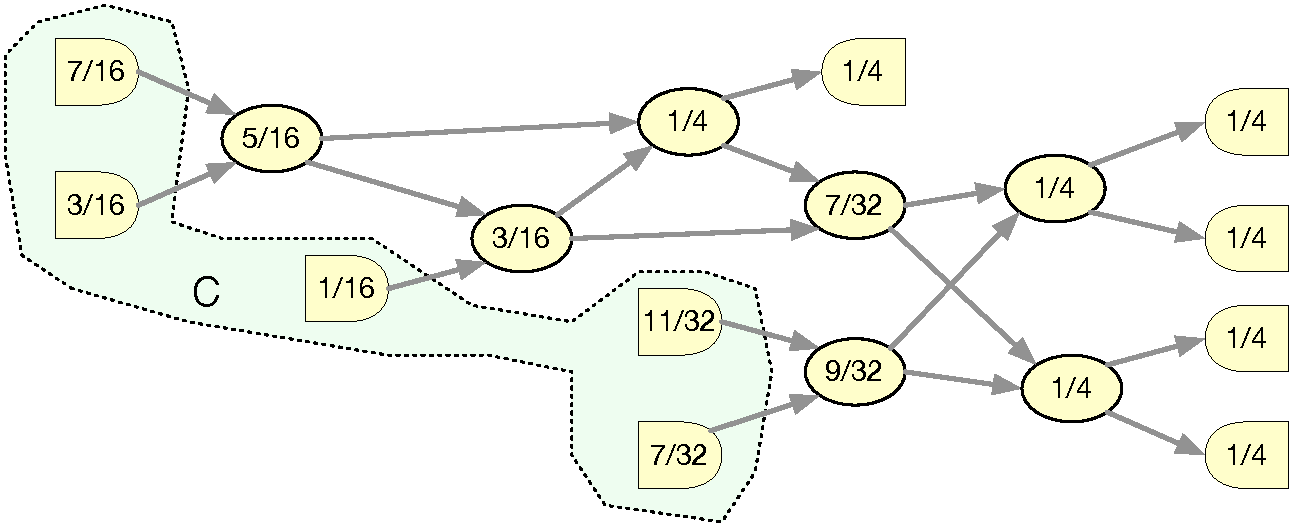
\includegraphics[width = 3.7in]{perfect_mixability_example.pdf}
		\caption{A mixing graph that perfectly mixes
		set $C = \braced{\onesixteenth, \threesixteenths,\seventhirtytwos,\eleventhirtytwos,\sevensixteenths}$.}
		\label{fig: dilution example}
	\end{center}
\end{figure}

Figure~\ref{fig: dilution example} shows an example of a perfect-mixing graph.
As an example of a set that is not perfectly mixable,
consider $D = \braced{0,\threesixteenths,\ninesixteenths}$. After any (non-zero) number of
mixing operations the resulting set of concentrations
will have the form $D' = \braced{a,a,b}$ for $a\neq b$, so no finite mixing graph will
convert $D$ into its perfect mixture $\braced{\onefourth,\onefourth,\onefourth}$.

In this paper, addressing the {\PerfectMixability} problem, 
we provide a complete characterization of perfectly mixable
droplet sets (with binary concentration values), and show that there is a polynomial-time 
algorithm that tests whether a given set is perfectly mixable,
and if so, constructs a polynomial-size perfect-mixing graph for it.

We represent droplet sets as multisets of concentration values.
First, we observe that without loss of generality we can assume that 
$C\cup\braced{\mu}\ingroundset \integers$, for otherwise we can simply 
rescale all values by an appropriate power of $2$. 
($\integers$ is the set of integers; $\posintegers$ and $\nonnegintegers$ are the sets of positive
and non-negative integers, respectively. Symbol $\ingroundset$ is used to specify a ground set of a multiset.)
For any finite multiset $A\ingroundset\integers$ and $b\in\posintegers$, we define
$A$ to be \emph{$b$-congruent} if $x\equiv y \pmod{b}$ for all $x,y\in A$.
(Otherwise we say that $A$ is \emph{$b$-incongruent}.)

We say that $C$ satisfies \emph{Condition~$\MixCond$} if, 
for each odd $b\in\posintegers$, if 
$C$ is $b$-congruent then $C\cup \braced{\mu}$ is $b$-congruent as well, 
where $\mu = \average(C)$.
The following theorem summarizes our results.

%%%%%%%%%%%%%%

\begin{theorem}\label{thm: miscibility characterization}
Assume that $n\ge 4$ and $C\cup \braced{\mu}\ingroundset\integers$, where 
$\mu = \average(C)$. Then:
\begin{description}
	\item[(a)] $C$ is perfectly mixable if and only if $C$ satisfies Condition~$\MixCond$.
	\item[(b)] If $C$ satisfies Condition~{\MixCond} then it can be perfectly mixed
	with precision at most $1$ and in a polynomial number of steps. 
	(That is, $C$ has a perfect-mixing graph of polynomial size where 
	all intermediate concentration values are half-integral.)
	\item[(c)] There is a polynomial-time algorithm that tests whether $C$ 
	is perfectly mixable and, if so, computes a polynomial-size perfect-mixing graph for $C$.
\end{description}
\end{theorem}

%%%%%%%%%%%%%%%%%

Part~(b) implies that, in general (if the concentrations in $C\cup\braced{\mu}$ are arbitrary
binary values), if $C$ is perfectly mixable at all then
$C$ can be mixed perfectly with precision at most
$d+1$, where $d$ is the maximum precision in $C\cup\braced{\mu}$; 
in other words, at most one extra bit of precision is needed
in the intermediate nodes of a perfect-mixing graph for $C$.

This extra 1-bit of precision in part~(b) of Theorem~\ref{thm: miscibility characterization}
is necessary. For example, $C = \braced{0,0,0,3,7}$ (for which $\mu = 2$) cannot be
mixed with precision $0$. If we mix $3$ and $7$, we will obtain multiset
$\braced{0,0,0,5,5}$ which is not perfectly mixable, as it violates Condition~{\MixCond}.
Any other mixing creates fractional values.
However, $C$ does have a mixing graph where the intermediate precision is at most $1$
--- see Figure~\ref{fig: precision 1 example}.


%%%%%%
	
\begin{figure}[ht]
	\begin{center}
		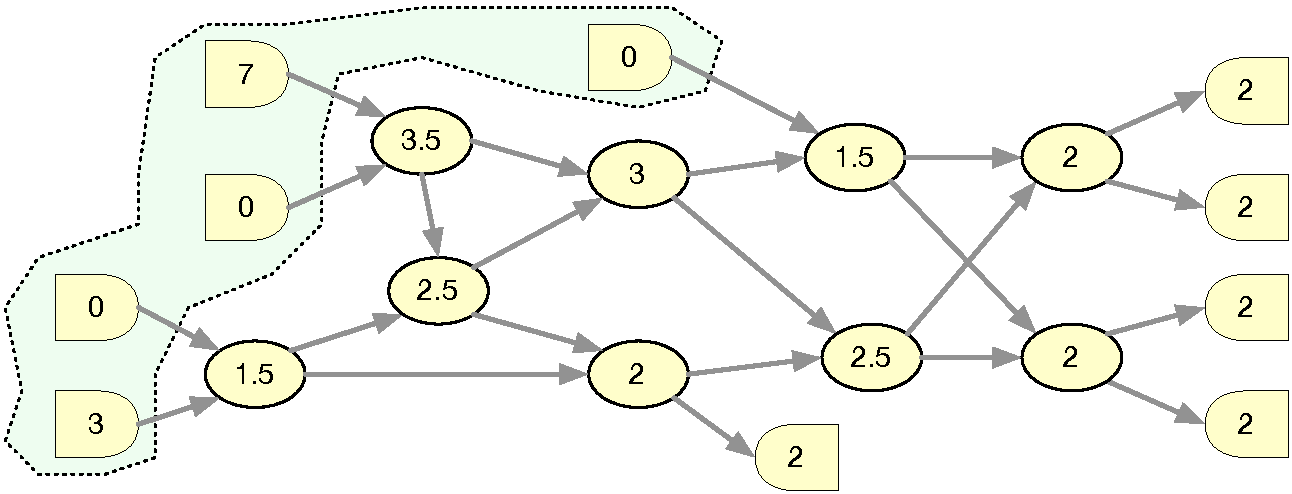
\includegraphics[width = 3.7in]{mixing_graph_example_precision1.pdf}
		\caption{A perfect mixing graph for $C = \braced{0,0,0,3,7}$ with precision $1$.}
		\label{fig: precision 1 example}
	\end{center}
\end{figure}

Note that in Theorem~\ref{thm: miscibility characterization} we assume that $n = |C|\ge 4$.
Regarding smaller values of $n$, for $n\leq 2$, trivially, all configurations $C$ with at most two droplets
are perfectly mixable with precision $0$.
The case $n=3$ is exceptional, as in this case
Theorem~\ref{thm: miscibility characterization} is actually false. (For example,
consider configuration $C = \braced{0,1,5}$, for which $\mu = 2$. This configuration
is $b$-incongruent for all odd $b>1$, so it satisfies condition~{\MixCond}, but is
not perfectly mixable.) 
Nevertheless, for $n=3$, perfectly mixable configurations are easy to
characterize: Let $C = \braced{a,b,c}$, where $a\le b \le c$.
Then $C$ is perfectly mixable if and only if $b = \half (a+c)$.
Further, if this condition holds, $C$ is perfectly mixable with precision $0$.
(That this condition is sufficient is obvious. That it is also necessary can
be proven by following the argument 
for the example configuration $D$ right after the definition of {\PerfectMixability}.)

To clarify the polynomial bounds in Theorem~\ref{thm: miscibility characterization},
we assume that the input configuration $C$ is specified by listing the concentration
values of individual droplets, and its size is the total number of bits
used in this representation. For the sake of concretness, we will
assume that $C$ is already rescaled to consist only of integers,
and we will define the input size as $s(C) = \sum_{c\in C}\log(|c|+2)$.
This value is within a small constant factor of the actual number of
bits representing $C$. 
Consequently, the polynomial bounds in Theorem~\ref{thm: miscibility characterization} 
are with respect to $s(C)$.

%%%%%%%%%%%%%%%%%%%%%


\myparagraph{Overview of the paper}
The proof of Theorem~\ref{thm: miscibility characterization}
is given in several sections. The necessity of Condition~{\MixCond} in 
Theorem~\ref{thm: miscibility characterization}(a)
is relatively simple to show; the proof appears in Section~\ref{sec: necessity of mc}. 
The proof that Condition~{\MixCond} is sufficient is more challenging. We first
show in Section~\ref{sec: some auxiliary lemmas} (see Corollary~\ref{cor: mc prime power factors})
that, in essence, in Condition~{\MixCond} it is sufficient to consider only
the values of $b$ that do not exceed the maximum concentration in $C$ and
are powers of prime factors of $n$.
This property is used in Section~\ref{sec: sufficiency of condition mc}
to show that any set $C$ that satisfies Condition~{\MixCond} has 
a perfect-mixing graph, completing the proof of Theorem~\ref{thm: miscibility characterization}(a).
The mixing graph constructed in Section~\ref{sec: sufficiency of condition mc} 
has precision at most $1$, proving the frst part of Theorem~\ref{thm: miscibility characterization}(b).
The second part, showing the existence of a perfect-mixing graph of polynomial
size is established in Section~\ref{sec: polynomial proof}.
The proof of Theorem~\ref{thm: miscibility characterization}(c) is divided into
two parts: that testing Condition~{\MixCond} can be done in polynomial
time follows directly from Corollary~\ref{cor: mc prime power factors} 
in Section~\ref{sec: some auxiliary lemmas}, while a polynomial-time 
algorithm for constructing a perfect-mixing graph is described
in Sections~\ref{sec: polynomial proof} and~\ref{sec: polynomial running time}.

